\documentclass[aspectratio=169, 11pt]{beamer}

% ========== 主题设置 ==========
\usetheme{Madrid}
\usecolortheme{whale}
\setbeamertemplate{navigation symbols}{}
\setbeamertemplate{footline}[frame number]

% ========== 包 ==========
\usepackage{tikz}
\usetikzlibrary{arrows.meta, positioning, shapes.geometric, calc, fit, backgrounds}
\usepackage{booktabs}
\usepackage{graphicx}
\usepackage{amsmath}
\usepackage{xcolor}

% ========== 颜色定义 ==========
\definecolor{highlight}{RGB}{255, 100, 100}      % 当前工作模块（红色高亮）
\definecolor{completed}{RGB}{100, 200, 100}      % 已完成模块（绿色）
\definecolor{pending}{RGB}{200, 200, 200}        % 待完成模块（灰色）
\definecolor{inprogress}{RGB}{100, 150, 255}     % 进行中（蓝色）

% ========== 标题信息 ==========
\title{Weekly Progress Report}
\subtitle{Week 26: Offline E2E Evaluation \& Final Report Draft Completion}
\author{Student ID: 11314389}
\institute{BCI Control System Project}
\date{March 17, 2026}

\begin{document}

% ========== 标题页 ==========
\begin{frame}
    \titlepage
\end{frame}

% ========== Slide 1: 系统架构图 ==========
\begin{frame}{System Overview: Current Focus}
    \begin{center}
    \resizebox{0.95\textwidth}{!}{%
    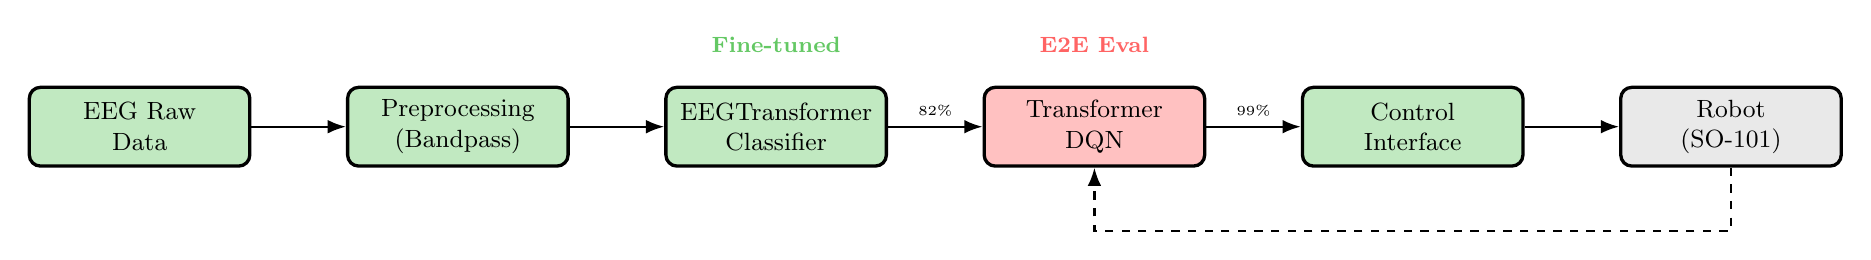
\begin{tikzpicture}[
        node distance=8mm and 12mm,
        block/.style={rectangle, rounded corners, draw, very thick,
                      minimum width=28mm, minimum height=10mm,
                      align=center, font=\small},
        arrow/.style={-Latex, thick},
    ]
        \node[block, fill=completed!40] (raw) {EEG Raw\\Data};
        \node[block, fill=completed!40, right=of raw] (prep) {Preprocessing\\(Bandpass)};
        \node[block, fill=completed!40, right=of prep] (ctnet) {EEGTransformer\\Classifier};
        \node[block, fill=highlight!40, right=of ctnet] (dqn) {Transformer\\DQN};
        \node[block, fill=completed!40, right=of dqn] (ctrl) {Control\\Interface};
        \node[block, fill=pending!40, right=of ctrl] (robot) {Robot\\(SO-101)};
        
        \draw[arrow] (raw) -- (prep);
        \draw[arrow] (prep) -- (ctnet);
        \draw[arrow] (ctnet) -- node[above, font=\tiny] {82\%} (dqn);
        \draw[arrow] (dqn) -- node[above, font=\tiny] {99\%} (ctrl);
        \draw[arrow] (ctrl) -- (robot);
        
        \draw[arrow, dashed] (robot.south) -- ++(0,-8mm) -| (dqn.south);
        
        \node[above=3mm of ctnet, completed, font=\footnotesize\bfseries] {Fine-tuned};
        \node[above=3mm of dqn, highlight, font=\footnotesize\bfseries] {E2E Eval};
        
    \end{tikzpicture}}
    \end{center}
    
    \vspace{3mm}
    \begin{columns}[T]
        \column{0.5\textwidth}
        \textbf{Legend:}
        \begin{itemize}
            \item[\textcolor{completed}{\rule{8pt}{8pt}}] Completed
            \item[\textcolor{inprogress}{\rule{8pt}{8pt}}] In Progress
        \end{itemize}
        \column{0.5\textwidth}
        \begin{itemize}
            \item[\textcolor{highlight}{\rule{8pt}{8pt}}] \textbf{This Week's Focus}
            \item[\textcolor{pending}{\rule{8pt}{8pt}}] Pending (Hardware)
        \end{itemize}
    \end{columns}
\end{frame}

% ========== Slide 2: 本周目标 ==========
\begin{frame}{This Week's Objectives}
    \begin{block}{Goals}
        \begin{enumerate}
            \item CTNet + DQN offline end-to-end evaluation (simulated)
            \item EEG-aware RL training comparison (with/without EEG input)
            \item ICA preprocessing comparison experiment
            \item Update final report with all experimental results (v4 $\rightarrow$ v6)
        \end{enumerate}
    \end{block}
    
    \vspace{5mm}
    
    \begin{alertblock}{Key Question to Address}
        Can the RL agent compensate for imperfect EEG classification (82\%) to achieve reliable robotic control?
    \end{alertblock}
\end{frame}

% ========== Slide 3: PhysioNet CTNet Training ==========
\begin{frame}{Background: PhysioNet CTNet Training}
    \begin{columns}[T]
        \column{0.55\textwidth}
        \textbf{Dataset: PhysioNet EEG Motor Movement/Imagery}
        \begin{itemize}
            \item 109 subjects, 64 channels, 160 Hz
            \item 4-class MI: Left hand, Right hand, Both feet, Both fists
            \item $\sim$90 trials per subject
        \end{itemize}
        
        \vspace{3mm}
        \textbf{Model: EEGTransformer (Hybrid CNN + Transformer)}
        \begin{itemize}
            \item EEGNet-style conv front-end for spatial filtering
            \item Multi-layer Transformer encoder for temporal modeling
            \item Residual fusion + classification head
        \end{itemize}
        
        \vspace{3mm}
        \textbf{Training Setup:}
        \begin{itemize}
            \item AdamW optimizer, cosine annealing LR
            \item Early stopping, 5-fold cross-validation
            \item InterAug data augmentation
        \end{itemize}
        
        \column{0.45\textwidth}
        \textbf{Results:}
        
        \vspace{1mm}
        \begin{table}
            \centering
            \small
            \begin{tabular}{lc}
                \toprule
                Configuration & Accuracy \\
                \midrule
                Cross-subject (109) & 56.54\% \\
                \textbf{+ Fine-tuning} & \textbf{88.78\%} \\
                \midrule
                Improvement & +32.24pp \\
                \bottomrule
            \end{tabular}
        \end{table}
        
        \vspace{1mm}
        \textbf{Per-Subject Fine-tuned Range:}
        \begin{itemize}
            \item Best: 97.78\% (S059)
            \item Worst: 75.56\% (S088)
            \item Reflects individual MI ability
        \end{itemize}
        
        \vspace{1mm}
        \begin{exampleblock}{Significance}
            Transfer learning enables fast adaptation with minimal calibration data
        \end{exampleblock}
    \end{columns}
\end{frame}

% ========== Slide 4: Channel Reduction Study ==========
\begin{frame}{Background: Channel Reduction Study}
    \begin{columns}[T]
        \column{0.55\textwidth}
        \textbf{Motivation:}
        \begin{itemize}
            \item OpenBCI Cyton only has 8 channels
            \item Need to reduce from 64 $\rightarrow$ 8 for deployment
            \item Which channels are most important?
        \end{itemize}
        
        \vspace{3mm}
        \textbf{Methodology:}
        \begin{itemize}
            \item Systematic ablation: 64 $\rightarrow$ 32 $\rightarrow$ 16 $\rightarrow$ 8
            \item Channel importance ranking via accuracy drop
            \item Focus on motor cortex region (C3, C4, Cz)
        \end{itemize}
        
        \vspace{3mm}
        \textbf{Key Finding:}
        \begin{alertblock}{C3 is Critical}
            Removing C3 causes largest accuracy drop ($-$8.3\%)\\
            Consistent with left motor cortex role in MI
        \end{alertblock}
        
        \column{0.45\textwidth}
        \textbf{Results by Channel Count:}
        
        \vspace{1mm}
        \begin{table}
            \centering
            \small
            \begin{tabular}{lcc}
                \toprule
                Channels & Cross-Sub & Fine-tuned \\
                \midrule
                64 (full) & 56.54\% & 88.78\% \\
                32 & 54.21\% & 85.43\% \\
                16 & 51.87\% & 80.12\% \\
                \textbf{8} & \textbf{48.92\%} & \textbf{72.54\%} \\
                \bottomrule
            \end{tabular}
        \end{table}
        
        \vspace{1mm}
        \textbf{Selected 8 Channels:}
        \begin{center}
            \texttt{C3, C4, Cz, FC3, FC4, CP3, CP4, Pz}
        \end{center}
        
        \vspace{1mm}
        \begin{exampleblock}{Conclusion}
            8-channel config retains 72.54\% accuracy\\
            Viable for OpenBCI deployment
        \end{exampleblock}
    \end{columns}
\end{frame}

% ========== Slide 5: E2E Evaluation 方法 ==========
\begin{frame}{Experiment 1: Offline E2E Evaluation (Simulated)}
    \begin{columns}[T]
        \column{0.55\textwidth}
        \textbf{Methodology:}
        \begin{enumerate}
            \item Load pre-trained CTNet (PhysioNet 109 subjects)
            \item Classify test subjects' EEG $\rightarrow$ 82.22\% accuracy
            \item Train Transformer DQN with/without EEG predictions
            \item Evaluate control in \textbf{PyBullet simulation} (not physical robot)
        \end{enumerate}
        
        \vspace{3mm}
        \textbf{Two Conditions:}
        \begin{itemize}
            \item \textbf{Arm state only}: 6D joint positions
            \item \textbf{Arm + EEG}: 6D + 4 class probs + confidence
        \end{itemize}
        
        \column{0.45\textwidth}
        \begin{center}
        \scalebox{0.9}{%
        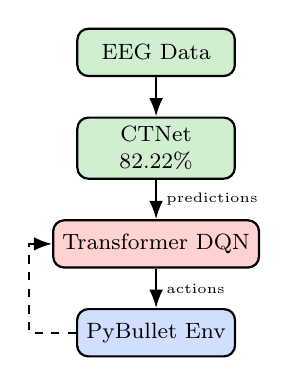
\begin{tikzpicture}[
            node distance=5mm,
            block/.style={rectangle, rounded corners, draw, thick,
                          minimum width=20mm, minimum height=6mm,
                          align=center, font=\footnotesize},
            arrow/.style={-Latex, thick},
        ]
            \node[block, fill=completed!30] (eeg) {EEG Data};
            \node[block, fill=completed!30, below=of eeg] (ctnet) {CTNet\\82.22\%};
            \node[block, fill=highlight!30, below=of ctnet] (dqn) {Transformer DQN};
            \node[block, fill=inprogress!30, below=of dqn] (env) {PyBullet Env};
            
            \draw[arrow] (eeg) -- (ctnet);
            \draw[arrow] (ctnet) -- node[right, font=\tiny] {predictions} (dqn);
            \draw[arrow] (dqn) -- node[right, font=\tiny] {actions} (env);
            \draw[arrow, dashed] (env.west) -- ++(-6mm,0) |- (dqn.west);
        \end{tikzpicture}}
        \end{center}
    \end{columns}
\end{frame}

% ========== Slide 6: E2E Results ==========
\begin{frame}{Experiment 1: Results -- RL Compensates in Simulation}
    \begin{columns}[T]
        \column{0.55\textwidth}
        \textbf{Performance Comparison:}
        
        \vspace{2mm}
        \begin{table}
            \centering
            \small
            \begin{tabular}{lcc}
                \toprule
                Metric & Arm Only & Arm + EEG \\
                \midrule
                Reach Rate & 99.0\% & 98.7\% \\
                Mean Reward & 91.2 & 90.8 \\
                Mean Steps & 18.7 & 19.1 \\
                \textbf{Train Time} & 1130s & \textbf{668s} \\
                \midrule
                \textbf{Speedup} & -- & \textbf{41\%} \\
                \bottomrule
            \end{tabular}
        \end{table}
        
        \vspace{3mm}
        \textbf{Key Insight:}
        \begin{itemize}
            \item Both achieve $\sim$99\% reach rate
            \item EEG input reduces training time by \textbf{41\%}
            \item RL compensates for 82\% $\rightarrow$ 99\% control
        \end{itemize}
        
        \column{0.45\textwidth}
        \begin{center}
        \textbf{Classification $\rightarrow$ Control}
        
        \vspace{3mm}
        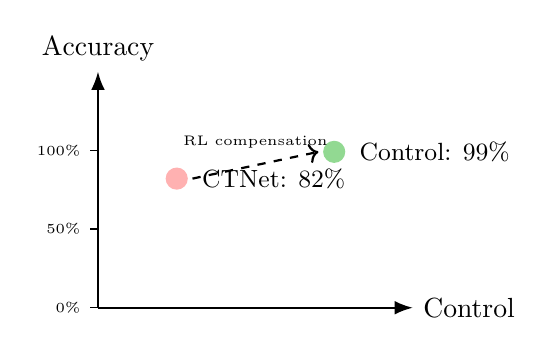
\begin{tikzpicture}
            \draw[thick, -Latex] (0,0) -- (4,0) node[right] {Control};
            \draw[thick, -Latex] (0,0) -- (0,3) node[above] {Accuracy};
            
            \fill[highlight!50] (1,1.64) circle (4pt);
            \node[right, font=\small] at (1.2,1.64) {CTNet: 82\%};
            
            \fill[completed!70] (3,1.98) circle (4pt);
            \node[right, font=\small] at (3.2,1.98) {Control: 99\%};
            
            \draw[thick, dashed, ->] (1.2,1.64) -- (2.8,1.98);
            \node[above, font=\tiny] at (2,1.9) {RL compensation};
            
            \foreach \y/\label in {0/0\%, 1/50\%, 2/100\%} {
                \draw (0,\y) -- (-0.1,\y) node[left, font=\tiny] {\label};
            }
        \end{tikzpicture}
        
        \vspace{5mm}
        \textit{RL learns to handle\\classification uncertainty}
        \end{center}
    \end{columns}
\end{frame}

% ========== Slide 5: ICA Experiment ==========
\begin{frame}{Experiment 2: ICA Preprocessing Comparison}
    \begin{columns}[T]
        \column{0.55\textwidth}
        \textbf{Methodology:}
        \begin{itemize}
            \item Dataset: BCI Competition IV-2a (MAT files)
            \item Compare: with ICA vs. without ICA
            \item ICA: FastICA, remove 2 highest-variance components
            \item 3 subjects tested (S1, S3, S7)
        \end{itemize}
        
        \vspace{3mm}
        \textbf{Results:}
        \begin{table}
            \centering
            \small
            \begin{tabular}{lccc}
                \toprule
                Subject & No ICA & With ICA & Diff \\
                \midrule
                S1 & 77.78\% & 75.00\% & \textcolor{red}{-2.78\%} \\
                S3 & 86.11\% & 87.50\% & \textcolor{completed}{+1.39\%} \\
                S7 & 69.44\% & 75.00\% & \textcolor{completed}{+5.56\%} \\
                \midrule
                \textbf{Avg} & 77.78\% & 79.17\% & \textbf{+1.51\%} \\
                \bottomrule
            \end{tabular}
        \end{table}
        
        \column{0.45\textwidth}
        \textbf{Key Findings:}
        
        \vspace{3mm}
        \begin{alertblock}{Marginal \& Inconsistent}
            \begin{itemize}
                \item Average gain: only +1.51\%
                \item S1 actually \textbf{degraded}
                \item 8--30Hz bandpass already removes most ocular artifacts
            \end{itemize}
        \end{alertblock}
        
        \vspace{3mm}
        \begin{exampleblock}{Decision}
            \textbf{Exclude ICA} from standard pipeline
            \begin{itemize}
                \item Adds complexity
                \item Inconsistent benefit
                \item Risk of removing signal
            \end{itemize}
        \end{exampleblock}
    \end{columns}
\end{frame}

% ========== Slide 6: Fine-tuning 原理 ==========
\begin{frame}{Transfer Learning: Fine-tuning Mechanism}
    \begin{columns}[T]
        \column{0.5\textwidth}
        \textbf{Two-Stage Training:}
        
        \vspace{2mm}
        \textbf{Stage 1: Cross-Subject Pre-training}
        \begin{itemize}
            \item Train on 109 subjects (PhysioNet)
            \item Learn population-level MI patterns
            \item Result: 56.54\% cross-subject accuracy
        \end{itemize}
        
        \vspace{3mm}
        \textbf{Stage 2: Subject-Specific Fine-tuning}
        \begin{itemize}
            \item Adapt to individual's neural signature
            \item Lower learning rate ($1\times10^{-4}$)
            \item Only $\sim$90 trials needed
            \item Result: \textbf{88.78\%} accuracy (+32pp)
        \end{itemize}
        
        \column{0.5\textwidth}
        \begin{center}
        \textbf{Why Fine-tuning Works}
        
        \vspace{3mm}
        \resizebox{\textwidth}{!}{%
        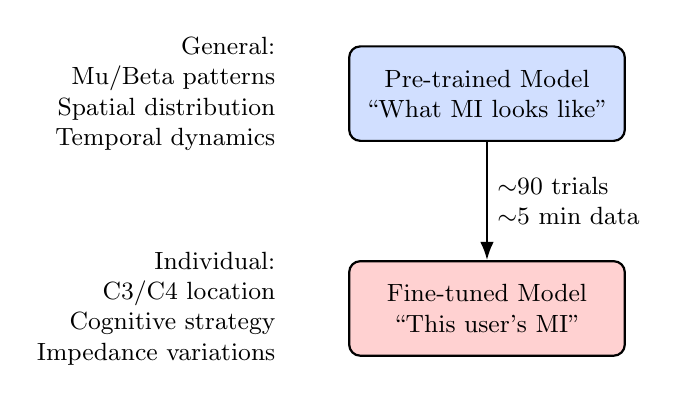
\begin{tikzpicture}[
            node distance=8mm,
            block/.style={rectangle, rounded corners, draw, thick,
                          minimum width=35mm, minimum height=12mm,
                          align=center, font=\small},
            arrow/.style={-Latex, thick},
        ]
            \node[block, fill=inprogress!30] (pretrain) {Pre-trained Model\\``What MI looks like''};
            \node[block, fill=highlight!30, below=15mm of pretrain] (finetune) {Fine-tuned Model\\``This user's MI''};
            
            \draw[arrow] (pretrain) -- node[right, font=\small, align=left] {$\sim$90 trials\\$\sim$5 min data} (finetune);
            
            \node[left=8mm of pretrain, font=\small, align=right] {General:\\Mu/Beta patterns\\Spatial distribution\\Temporal dynamics};
            
            \node[left=8mm of finetune, font=\small, align=right] {Individual:\\C3/C4 location\\Cognitive strategy\\Impedance variations};
        \end{tikzpicture}}
        
        \vspace{5mm}
        \textit{Model already knows MI structure;\\only needs to adapt to individual}
        \end{center}
    \end{columns}
\end{frame}

% ========== Slide 7: 部署流程 ==========
\begin{frame}{Deployment Workflow: Three Phases}
    \begin{center}
    \resizebox{0.95\textwidth}{!}{%
    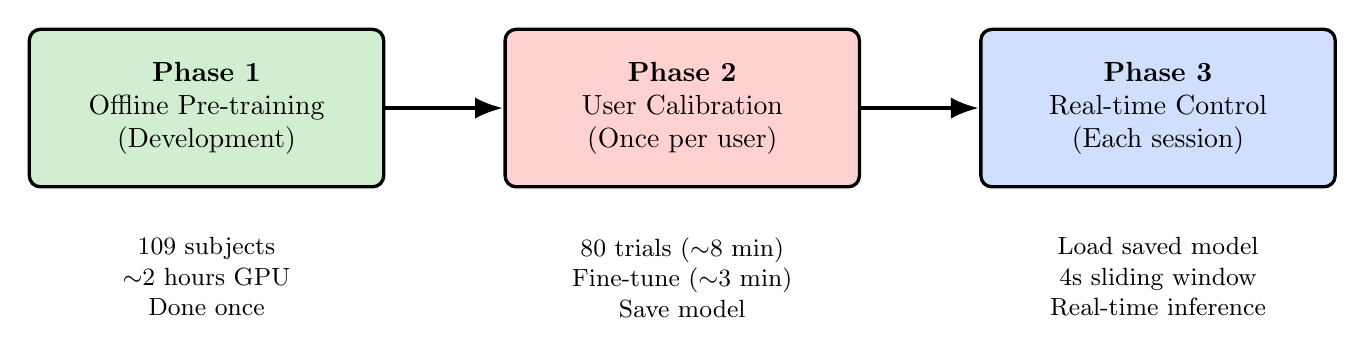
\begin{tikzpicture}[
        node distance=15mm,
        phase/.style={rectangle, rounded corners, draw, very thick,
                      minimum width=45mm, minimum height=20mm,
                      align=center, font=\normalsize},
        arrow/.style={-Latex, ultra thick},
    ]
        \node[phase, fill=completed!30] (p1) {\textbf{Phase 1}\\Offline Pre-training\\(Development)};
        \node[phase, fill=highlight!30, right=of p1] (p2) {\textbf{Phase 2}\\User Calibration\\(Once per user)};
        \node[phase, fill=inprogress!30, right=of p2] (p3) {\textbf{Phase 3}\\Real-time Control\\(Each session)};
        
        \draw[arrow] (p1) -- (p2);
        \draw[arrow] (p2) -- (p3);
        
        \node[below=5mm of p1, font=\small, align=center] {109 subjects\\$\sim$2 hours GPU\\Done once};
        \node[below=5mm of p2, font=\small, align=center] {80 trials ($\sim$8 min)\\Fine-tune ($\sim$3 min)\\Save model};
        \node[below=5mm of p3, font=\small, align=center] {Load saved model\\4s sliding window\\Real-time inference};
    \end{tikzpicture}}
    \end{center}
    
    \vspace{5mm}
    \begin{columns}[T]
        \column{0.5\textwidth}
        \textbf{Total Setup Time per User:}
        \begin{itemize}
            \item Data collection: $\sim$8 minutes
            \item Fine-tuning: $\sim$3 minutes (GPU)
            \item \textbf{Total: $\sim$11 minutes}
        \end{itemize}
        
        \column{0.5\textwidth}
        \textbf{Comparable to Commercial BCIs:}
        \begin{itemize}
            \item Emotiv: 10--15 min calibration
            \item NeuroSky: 5--10 min setup
            \item Our system: 11 min (one-time)
        \end{itemize}
    \end{columns}
\end{frame}

% ========== Slide 8: Final Report Updates ==========
\begin{frame}{Final Report: v4 $\rightarrow$ v6 Updates}
    \begin{columns}[T]
        \column{0.5\textwidth}
        \textbf{v4 $\rightarrow$ v5 (Fine-tuning Details):}
        \begin{itemize}
            \item Training Strategy: two-stage protocol
            \item Real-Time Pipeline: three-phase deployment
            \item Discussion: why fine-tuning works
            \item Limitations: 10-subject validation note
        \end{itemize}
        
        \vspace{3mm}
        \textbf{v5 $\rightarrow$ v6 (Hardware Status):}
        \begin{itemize}
            \item New section: ``Hardware Validation Status''
            \item Clarify what's completed vs. pending
            \item Updated conclusion with next steps
        \end{itemize}
        
        \column{0.5\textwidth}
        \textbf{Hardware Validation Status:}
        
        \vspace{2mm}
        \begin{exampleblock}{Completed (Software)}
            \begin{itemize}
                \item EEGTransformer on 3 datasets
                \item DQN in PyBullet (99\% reach)
                \item BrainFlow API integration
                \item SO-101 serial protocol
            \end{itemize}
        \end{exampleblock}
        
        \begin{alertblock}{Pending (Hardware)}
            \begin{itemize}
                \item Live human subject testing
                \item OpenBCI + SO-101 closed loop
                \item Scheduled with supervisor
            \end{itemize}
        \end{alertblock}
    \end{columns}
\end{frame}

% ========== Slide 9: 实验结果汇总 ==========
\begin{frame}{Summary: All Experimental Results}
    \begin{table}
        \centering
        \small
        \begin{tabular}{llc}
            \toprule
            \textbf{Experiment} & \textbf{Key Finding} & \textbf{Status} \\
            \midrule
            Cross-subject CTNet & 56.54\% (109 subjects) & \textcolor{completed}{\checkmark} \\
            Fine-tuned CTNet & 88.78\% (+32pp) & \textcolor{completed}{\checkmark} \\
            Channel Reduction & 8-ch: 72.54\% (viable) & \textcolor{completed}{\checkmark} \\
            Simulated E2E Control & 82\% class $\rightarrow$ 99\% control & \textcolor{completed}{\checkmark} \\
            EEG-aware Training & 41\% faster training & \textcolor{completed}{\checkmark} \\
            ICA Comparison & +1.51\% (excluded) & \textcolor{completed}{\checkmark} \\
            \midrule
            Physical Robot Test & Pending hardware & \textcolor{pending}{$\circ$} \\
            \bottomrule
        \end{tabular}
    \end{table}
    
    \vspace{5mm}
    \begin{center}
    \textbf{All software experiments completed.}\\
    \textbf{Hardware validation is the only remaining task.}
    \end{center}
\end{frame}

% ========== Slide 10: 下周计划 ==========
\begin{frame}{Next Steps: Hardware Validation}
    \begin{block}{Priority Tasks (Pending Hardware Access)}
        \begin{enumerate}
            \item Validate 8-channel OpenBCI configuration with live subject
            \item Measure real-time classification latency
            \item End-to-end closed-loop test: EEG $\rightarrow$ CTNet $\rightarrow$ DQN $\rightarrow$ SO-101
            \item Qualitative usability assessment
        \end{enumerate}
    \end{block}
    
    \vspace{5mm}
    
    \begin{columns}[T]
        \column{0.5\textwidth}
        \textbf{Hardware Requirements:}
        \begin{itemize}
            \item OpenBCI Cyton (8-channel)
            \item SO-101 robotic arm
            \item Participant recruitment
            \item Safety protocol approval
        \end{itemize}
        
        \column{0.5\textwidth}
        \textbf{Questions for Supervisor:}
        \begin{itemize}
            \item Hardware session?
            \item Participant recruitment process?
            \item Safety/ethics approval status?
        \end{itemize}
    \end{columns}
\end{frame}

% ========== Slide 11: 时间线 ==========
\begin{frame}{Project Timeline}
    \begin{center}
    \resizebox{0.9\textwidth}{!}{%
    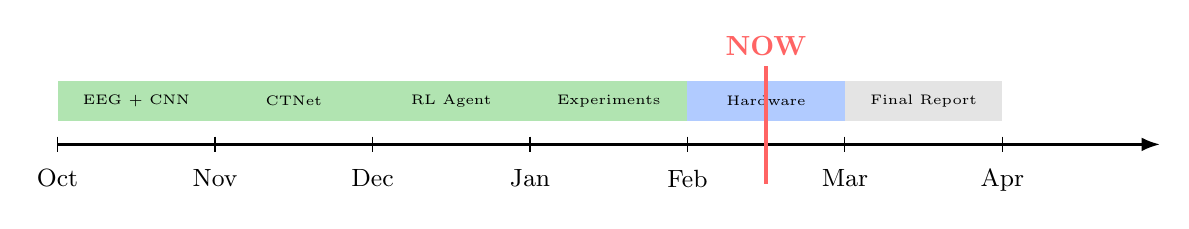
\begin{tikzpicture}
        \draw[thick, -Latex] (0,0) -- (14,0);
        
        \foreach \x/\month in {0/Oct, 2/Nov, 4/Dec, 6/Jan, 8/Feb, 10/Mar, 12/Apr} {
            \draw (\x, 0.1) -- (\x, -0.1);
            \node[below] at (\x, -0.2) {\small \month};
        }
        
        \fill[completed!50] (0, 0.3) rectangle (2, 0.8);
        \node at (1, 0.55) {\tiny EEG + CNN};
        
        \fill[completed!50] (2, 0.3) rectangle (4, 0.8);
        \node at (3, 0.55) {\tiny CTNet};
        
        \fill[completed!50] (4, 0.3) rectangle (6, 0.8);
        \node at (5, 0.55) {\tiny RL Agent};
        
        \fill[completed!50] (6, 0.3) rectangle (8, 0.8);
        \node at (7, 0.55) {\tiny Experiments};
        
        \fill[inprogress!50] (8, 0.3) rectangle (10, 0.8);
        \node at (9, 0.55) {\tiny Hardware};
        
        \fill[pending!50] (10, 0.3) rectangle (12, 0.8);
        \node at (11, 0.55) {\tiny Final Report};
        
        \draw[highlight, ultra thick] (9, -0.5) -- (9, 1);
        \node[highlight, above] at (9, 1) {\textbf{NOW}};
        
    \end{tikzpicture}}
    \end{center}
    
    \vspace{3mm}
    \textbf{Current Status:} On track -- all software work completed
    
    \textbf{This Week's Achievement:} Offline E2E evaluation shows 82\% $\rightarrow$ 99\% control (simulated)
\end{frame}

% ========== Slide 12: Summary ==========
\begin{frame}{Summary}
    \begin{center}
    \Large
    \textbf{Key Achievements This Week}
    \end{center}
    
    \vspace{5mm}
    
    \begin{enumerate}
        \item \textbf{Offline E2E Evaluation}: RL compensates 82\% classification $\rightarrow$ 99\% control (simulated)
        \item \textbf{EEG-aware Training}: 41\% faster convergence with EEG input
        \item \textbf{ICA Decision}: Excluded from pipeline (marginal +1.51\%, inconsistent)
        \item \textbf{Fine-tuning Analysis}: $\sim$11 min calibration enables 88.78\% accuracy
        \item \textbf{Report v6}: Complete with hardware status clarification
    \end{enumerate}
    
    \vspace{10mm}
    
    \begin{center}
    \textit{All software experiments completed.}\\
    \textit{Ready for hardware validation when equipment available.}
    \end{center}
\end{frame}

\end{document}
